% Choose one to switch betweeen slides and handout
\documentclass[]{beamer}
%\documentclass[handout]{beamer}

% Video Meta Data
\title{Bitcoin, Blockchain and Cryptoassets}
\subtitle{Bitcoin Primer}
\author{Prof. Dr. Fabian Schär}
\institute{University of Basel}

% Config File
% Packages
\usepackage[utf8]{inputenc}
\usepackage{hyperref}
\usepackage{gitinfo2}
\usepackage{tikz}
\usepackage{amsmath}
\usepackage{bibentry}
\usepackage{xcolor}
\usepackage{colortbl} % Add colour to LaTeX tables
\usepackage{caption}
\usepackage[export]{adjustbox}
\usepackage{pgfplots} \pgfplotsset{compat = 1.17}

% Color Options
\definecolor{highlight}{rgb}{0.65,0.84,0.82}
\definecolor{focus}{rgb}{0.72, 0, 0}

% Beamer Template Options
\beamertemplatenavigationsymbolsempty
\setbeamertemplate{footline}[frame number]
\setbeamercolor{structure}{fg=black}
\setbeamercolor{footline}{fg=black}
\setbeamercolor{title}{fg=black}
\setbeamercolor{frametitle}{fg=black}
\setbeamercolor{item}{fg=black}
\setbeamercolor{}{fg=black}
\setbeamercolor{bibliography item}{fg=black}
\setbeamercolor*{bibliography entry title}{fg=black}
\setbeamertemplate{items}[square]
\setbeamertemplate{enumerate items}[default]
\captionsetup[figure]{labelfont={color=black},font={color=black}}
\captionsetup[table]{labelfont={color=black},font={color=black}}

\setbeamertemplate{bibliography item}{\insertbiblabel}

% Link Icon Command
\newcommand{\link}{%
    \tikz[x=1.2ex, y=1.2ex, baseline=-0.05ex]{%
        \begin{scope}[x=1ex, y=1ex]
            \clip (-0.1,-0.1)
                --++ (-0, 1.2)
                --++ (0.6, 0)
                --++ (0, -0.6)
                --++ (0.6, 0)
                --++ (0, -1);
            \path[draw,
                line width = 0.5,
                rounded corners=0.5]
                (0,0) rectangle (1,1);
        \end{scope}
        \path[draw, line width = 0.5] (0.5, 0.5)
            -- (1, 1);
        \path[draw, line width = 0.5] (0.6, 1)
            -- (1, 1) -- (1, 0.6);
        }
    }

% Read Git Data from Github Actions Workflow
% Defaults to gitinfo2 for local builds
\IfFileExists{gitInfo.txt}
	{\input{gitInfo.txt}}
	{
		\newcommand{\gitRelease}{(Local Release)}
		\newcommand{\gitSHA}{\gitHash}
		\newcommand{\gitDate}{\gitAuthorIsoDate}
	}

% Custom Titlepage
\defbeamertemplate*{title page}{customized}[1][]
{
  \vspace{-0cm}\hfill
\includegraphics[width=2.5cm]{../config/logo_cif}
  
\includegraphics[width=1.9cm]{../config/seal_wwz}
  \\ \vspace{2em}
  \usebeamerfont{title}\textbf{\inserttitle}\par
  \usebeamerfont{title}\usebeamercolor[fg]{title}\insertsubtitle\par  \vspace{1.5em}
  \small\usebeamerfont{author}\insertauthor\par
  \usebeamerfont{author}\insertinstitute\par \vspace{2em}
  \usebeamercolor[fg]{titlegraphic}\inserttitlegraphic
    \tiny \noindent \texttt{Release Ver.: \gitRelease}\\ 
    \texttt{Version Hash: \gitSHA}\\
    \texttt{Version Date: \gitDate}\\ \vspace{1em}
  \link \href{https://github.com/cifunibas/Bitcoin-Blockchain-Cryptoassets/blob/main/slides/intro.pdf}
  {Get most recent version}\\
  \link \href{https://github.com/cifunibas/Bitcoin-Blockchain-Cryptoassets/blob/main/slides/intro.pdf}
  {Watch video lecture}\\ \vspace{1em}
  License: \texttt{Creative Commons Attribution-NonCommercial-ShareAlike 4.0 International}\\\vspace{2em}
  
\includegraphics[width = 1.2cm]{../config/license}
}

% tikzlibraries
\usetikzlibrary{decorations.pathreplacing}
\usetikzlibrary{decorations.markings}
\usetikzlibrary{positioning}

%caption font
\captionsetup{font=footnotesize}

%%%%%%%%%%%%%%%%%%%%%%%%%%%%%%%%%%%%%%%%%%%%%%
%%%%%%%%%%%%%%%%%%%%%%%%%%%%%%%%%%%%%%%%%%%%%%
\begin{document}

\thispagestyle{empty}
\begin{frame}[noframenumbering]
	\titlepage
\end{frame}

%%%
\begin{frame}{Definition}
Some key aspects of Bitcoin: \vspace{1em}

	\begin{enumerate}
		\item<2-> competitively created
		\item<3-> virtually represented
		\item<4-> decentrally managed
	\end{enumerate}
	\vspace{1em}	
\uncover<5->{Bitcoin is a decentrally managed and unique public database.} \\	 			\vspace{1em}
\uncover<6->{The innovation of bitcoin is the conscious ommission of central actors.} %and 		minimal dependencies on 3rd parties
\end{frame}
%%%	

%%%
\begin{frame}{Bitcoin building blocks}
%%
\begin{figure}[h!]
  \center
  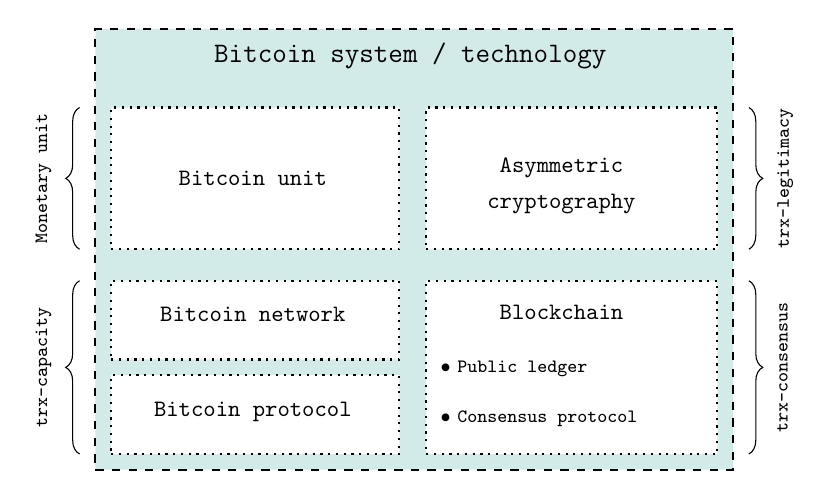
\begin{tikzpicture}[domain=0:10,scale=0.8, every node/.style={scale=0.85}]
    \draw[dashed, thick, fill=highlight!50] (0,0) -- (10.125,0) -- (10.125,7) -- (0,7) -- (0,0);
    

    \draw[dotted, thick,fill=white] (0.25,0.25) -- (4.825,0.25) -- (4.825,1.5) -- (0.25,1.5) -- (0.25,0.25);  
    \draw[color=black] (2.5,0.925) node{\texttt{Bitcoin protocol}};
    
    \draw[dotted, thick,fill=white] (0.25,1.75) -- (4.825,1.75) -- (4.825,3) -- (0.25,3) -- (0.25,1.75);
    \draw[color=black] (2.5,2.475) node{\texttt{Bitcoin network}};  
        
    \draw[dotted, thick,fill=white] (0.25,3.5) -- (4.825,3.5) -- (4.825,5.75) -- (0.25,5.75) -- (0.25,3.5);
    \draw[color=black] (2.5,4.625) node{\texttt{Bitcoin unit}};    
    
    \draw[dotted, thick,fill=white] (5.25,0.25) -- (9.875,0.25) -- (9.875,3) -- (5.25,3) -- (5.25,0.25);
    \draw[color=black] (7.4,2.25) node[above]{\texttt{Blockchain}};   
    \draw[color=black] (5.35,1.6) node[right]{\footnotesize{$\bullet$ \texttt{Public ledger}}};   
    \draw[color=black] (5.35,0.8) node[right]{\footnotesize{$\bullet$ \texttt{Consensus protocol}}};
    
    \draw[dotted, thick,fill=white] (5.25,3.5) -- (9.875,3.5) -- (9.875,5.75) -- (5.25,5.75) -- (5.25,3.5);
    \draw[color=black] (7.4,4.5) node[above]{\texttt{Asymmetric}} node[below]{\texttt{cryptography}};      

    \draw (5,6.9)node[below]{\large{\texttt{Bitcoin system / technology}}};
    
    \draw [decorate,decoration={brace,amplitude=5pt},xshift=0pt,yshift=0pt]
  	(-0.25,0.25) -- (-0.25,3) node [above,black,midway,xshift=-0.3cm,rotate=90]{\footnotesize \texttt{trx-capacity}};

    \draw [decorate,decoration={brace,amplitude=5pt,mirror},xshift=0pt,yshift=0pt]
 	(10.375,0.25) -- (10.375,3) node [below,black,midway,xshift=0.3cm,rotate=90] 
 	{\footnotesize \texttt{trx-consensus}};

    \draw [decorate,decoration={brace,amplitude=5pt},xshift=0pt,yshift=0pt]
	(-0.25,3.5) -- (-0.25,5.75) node [above,black,midway,xshift=-0.3cm,rotate=90] 
	{\footnotesize \texttt{Monetary unit}};

   	\draw [decorate,decoration={brace,amplitude=5pt,mirror},xshift=0pt,yshift=0pt]
	(10.375,3.5) -- (10.375,5.75) node [below,black,midway,xshift=0.3cm,rotate=90] 
	{\footnotesize \texttt{trx-legitimacy}};
    
  \end{tikzpicture}
  %\caption{Overview Bitcoin-system (trx = transaction)}
  \label{fig:bitcoinsystem}
\end{figure}
%%
\begin{center}
\uncover<2->{
Because of the decentralized infrastructure, the transaction \textbf{capacity}, transaction \textbf{legitimacy} and transaction \textbf{consensus} are much more difficult to achieve.
}
\end{center}
\end{frame}
%%%

%%%
\begin{frame}{Transaction capacity}
\textbf{Goal:} ensuring the ability to initiate a transaction  \\
\vspace{1em}
\uncover<2->{Bitcoin network 
        \begin{itemize}
		\item {consists of all users}
		\item {primary communication path}
		%\item<2->{completely decentral}
		\end{itemize}
		}
\vspace{1em}
\uncover<3->{Bitcoin protocol
        \begin{itemize}
        \item<3->{defines manner (ruleset) in which communication has to take place}
        \end{itemize}
        }     
\end{frame}
%%%


%%%
\begin{frame}{Transaction capacity}  %example banking vs. decentral system?

{\begin{figure}[h!]
\center
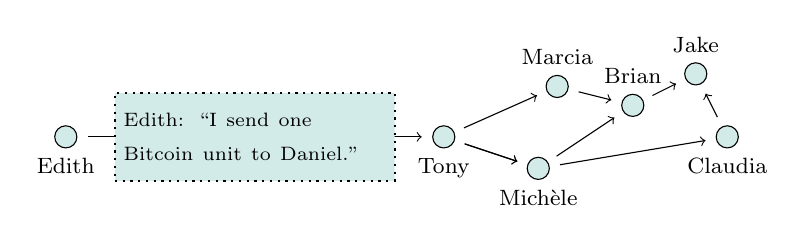
\begin{tikzpicture}[domain=-8:8, scale=0.8]
\coordinate (c1) at (0,0);
\coordinate (c2) at (6,0);
\coordinate (c3) at (7.8,0.8);
\coordinate (c4) at (7.5,-0.5);
\coordinate (c5) at (9,0.5);
\coordinate (c6) at (10,1);
\coordinate (c7) at (10.5,0);
\filldraw[draw=black,fill=highlight!50] (c1) circle (5pt) node[below=0.15cm,color=black]{\footnotesize{Edith}};
\filldraw[draw=black,fill=highlight!50] (c2) circle (5pt) node[below=0.15cm,color=black]{\footnotesize{Tony}};
\filldraw[draw=black,fill=highlight!50] (c3) circle (5pt) node[above=0.15cm,color=black]{\footnotesize{Marcia}};
\filldraw[draw=black,fill=highlight!50] (c4) circle (5pt) node[below=0.15cm,color=black]{\footnotesize{Michèle}};
\filldraw[draw=black,fill=highlight!50] (c5) circle (5pt) node[above=0.15cm,color=black]{\footnotesize{Brian}};
\filldraw[draw=black,fill=highlight!50] (c6) circle (5pt) node[above=0.15cm,color=black]{\footnotesize{Jake}};
\filldraw[draw=black,fill=highlight!50] (c7) circle (5pt) node[below=0.15cm,color=black]{\footnotesize{Claudia}};

\draw[shorten >=0.28cm,shorten <=0.28cm,->] (c1) to[] (c2);
\draw[shorten >=0.28cm,shorten <=0.28cm,->] (c2) to[] (c3);
\draw[shorten >=0.28cm,shorten <=0.28cm,->] (c2) to[] (c4);
\draw[shorten >=0.28cm,shorten <=0.28cm,->] (c2) to[] (c4);
\draw[shorten >=0.28cm,shorten <=0.28cm,->] (c3) to[] (c5);
\draw[shorten >=0.28cm,shorten <=0.28cm,->] (c4) to[] (c5);
\draw[shorten >=0.28cm,shorten <=0.28cm,->] (c4) to[] (c7);
\draw[shorten >=0.28cm,shorten <=0.28cm,->] (c5) to[] (c6);
\draw[shorten >=0.28cm,shorten <=0.28cm,->] (c7) to[] (c6);

\filldraw[fill=highlight!50,dotted,thick] (0.78,-0.7) -- (5.22,-0.7) -- (5.22,0.7) -- (0.78,0.7) -- (0.78,-0.7) node[midway, right=-0.02cm,text width=4.25cm]{\scriptsize{Edith: ``I send one \\ Bitcoin unit to Daniel.''}};

\end{tikzpicture}
\end{figure}\vspace{1em}
}

\uncover<2->{        
        \begin{itemize}
		\item<1-> permissionless, censorship-resistant
		\item<1-> participants are equal
		\item<1-> peer-to-peer network %(an. Bit Torrent) %robust
		\end{itemize}
		}
\end{frame}
%%%


%%%
\begin{frame}{Transaction legitimacy}
\textbf{Goal:} ensuring that a transaction was initiated by the actual owner
	\vspace{1em}
\uncover<2->{
	\begin{figure}[h!]
\center
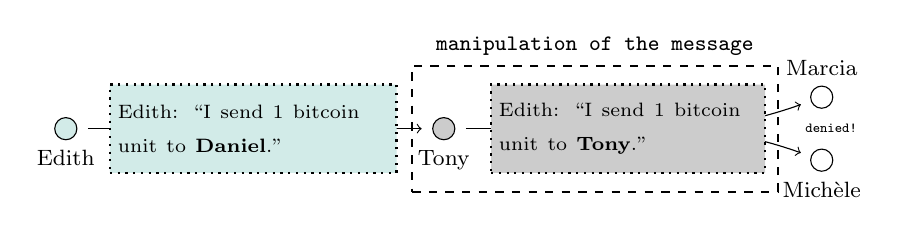
\begin{tikzpicture}[domain=-8:8, scale=0.8]
\coordinate (c1) at (0,0);
\coordinate (c2) at (6,0);
%\coordinate (c3) at (7.8,0.8);
%\coordinate (c4) at (7.5,-0.5);
%\coordinate (c5) at (9,0.5);
%\coordinate (c6) at (10,1);
%\coordinate (c7) at (10.5,0);
\filldraw[draw=black,fill=highlight!50] (c1) circle (5pt) node[below=0.15cm,color=black]{\footnotesize{Edith}};
\filldraw[draw=black,fill=black!20] (c2) circle (5pt) node[below=0.15cm,color=black]{\footnotesize{Tony}};

\draw[shorten >=0.28cm,shorten <=0.28cm,->] (c1) to[] (c2);
\draw[shorten >=0.28cm,shorten <=0.28cm,->] (c2) to[] (9,0);
\draw[shorten >=0.28cm,shorten <=0.28cm,->] (9,0) to[bend right = 10] (12,0.5);
\draw[shorten >=0.28cm,shorten <=0.28cm,->] (9,0) to[bend left = 10] (12,-0.5);

\filldraw[draw=black,fill=white] (12,0.5) circle (5pt) node[above=0.15cm,color=black]{\footnotesize{Marcia}};
\filldraw[draw=black,fill=white] (12,-0.5) circle (5pt) node[below=0.15cm,color=black]{\footnotesize{Michèle}};


\filldraw[fill=highlight!50,dotted,thick] (0.7,-0.7) -- (5.25,-0.7) -- (5.25,0.7) -- (0.7,0.7) -- (0.7,-0.7) node[midway, right=-0.03cm,text width=3.5cm]{\scriptsize{Edith: ``I send 1 bitcoin unit to \textbf{Daniel}.''}};

\filldraw[fill=black!20,dotted,thick] (6.75,-0.7) -- (11.1,-0.7) -- (11.1,0.7) -- (6.75,0.7) -- (6.75,-0.7) node[midway, right=-0.03cm,text width=3.3cm]{\scriptsize{Edith: ``I send 1 bitcoin unit to \textbf{Tony}.''}};

\draw[dashed, thick] (5.5,-1) -- (11.3,-1) -- (11.3,1) -- (5.5,1) node[midway,above]{\footnotesize{\texttt{manipulation of the message}}} -- (5.5,-1) ;

\draw (12.15,0) node[color=black]{\tiny{\texttt{denied!}}};

\end{tikzpicture}
\end{figure}
	\vspace{2em}
\textbf{Tool:} asymmetric cryptography
	}
\end{frame}
%%%


%%%
\begin{frame}{Blocks and the blockchain}
Transactions are bundled into blocks \\
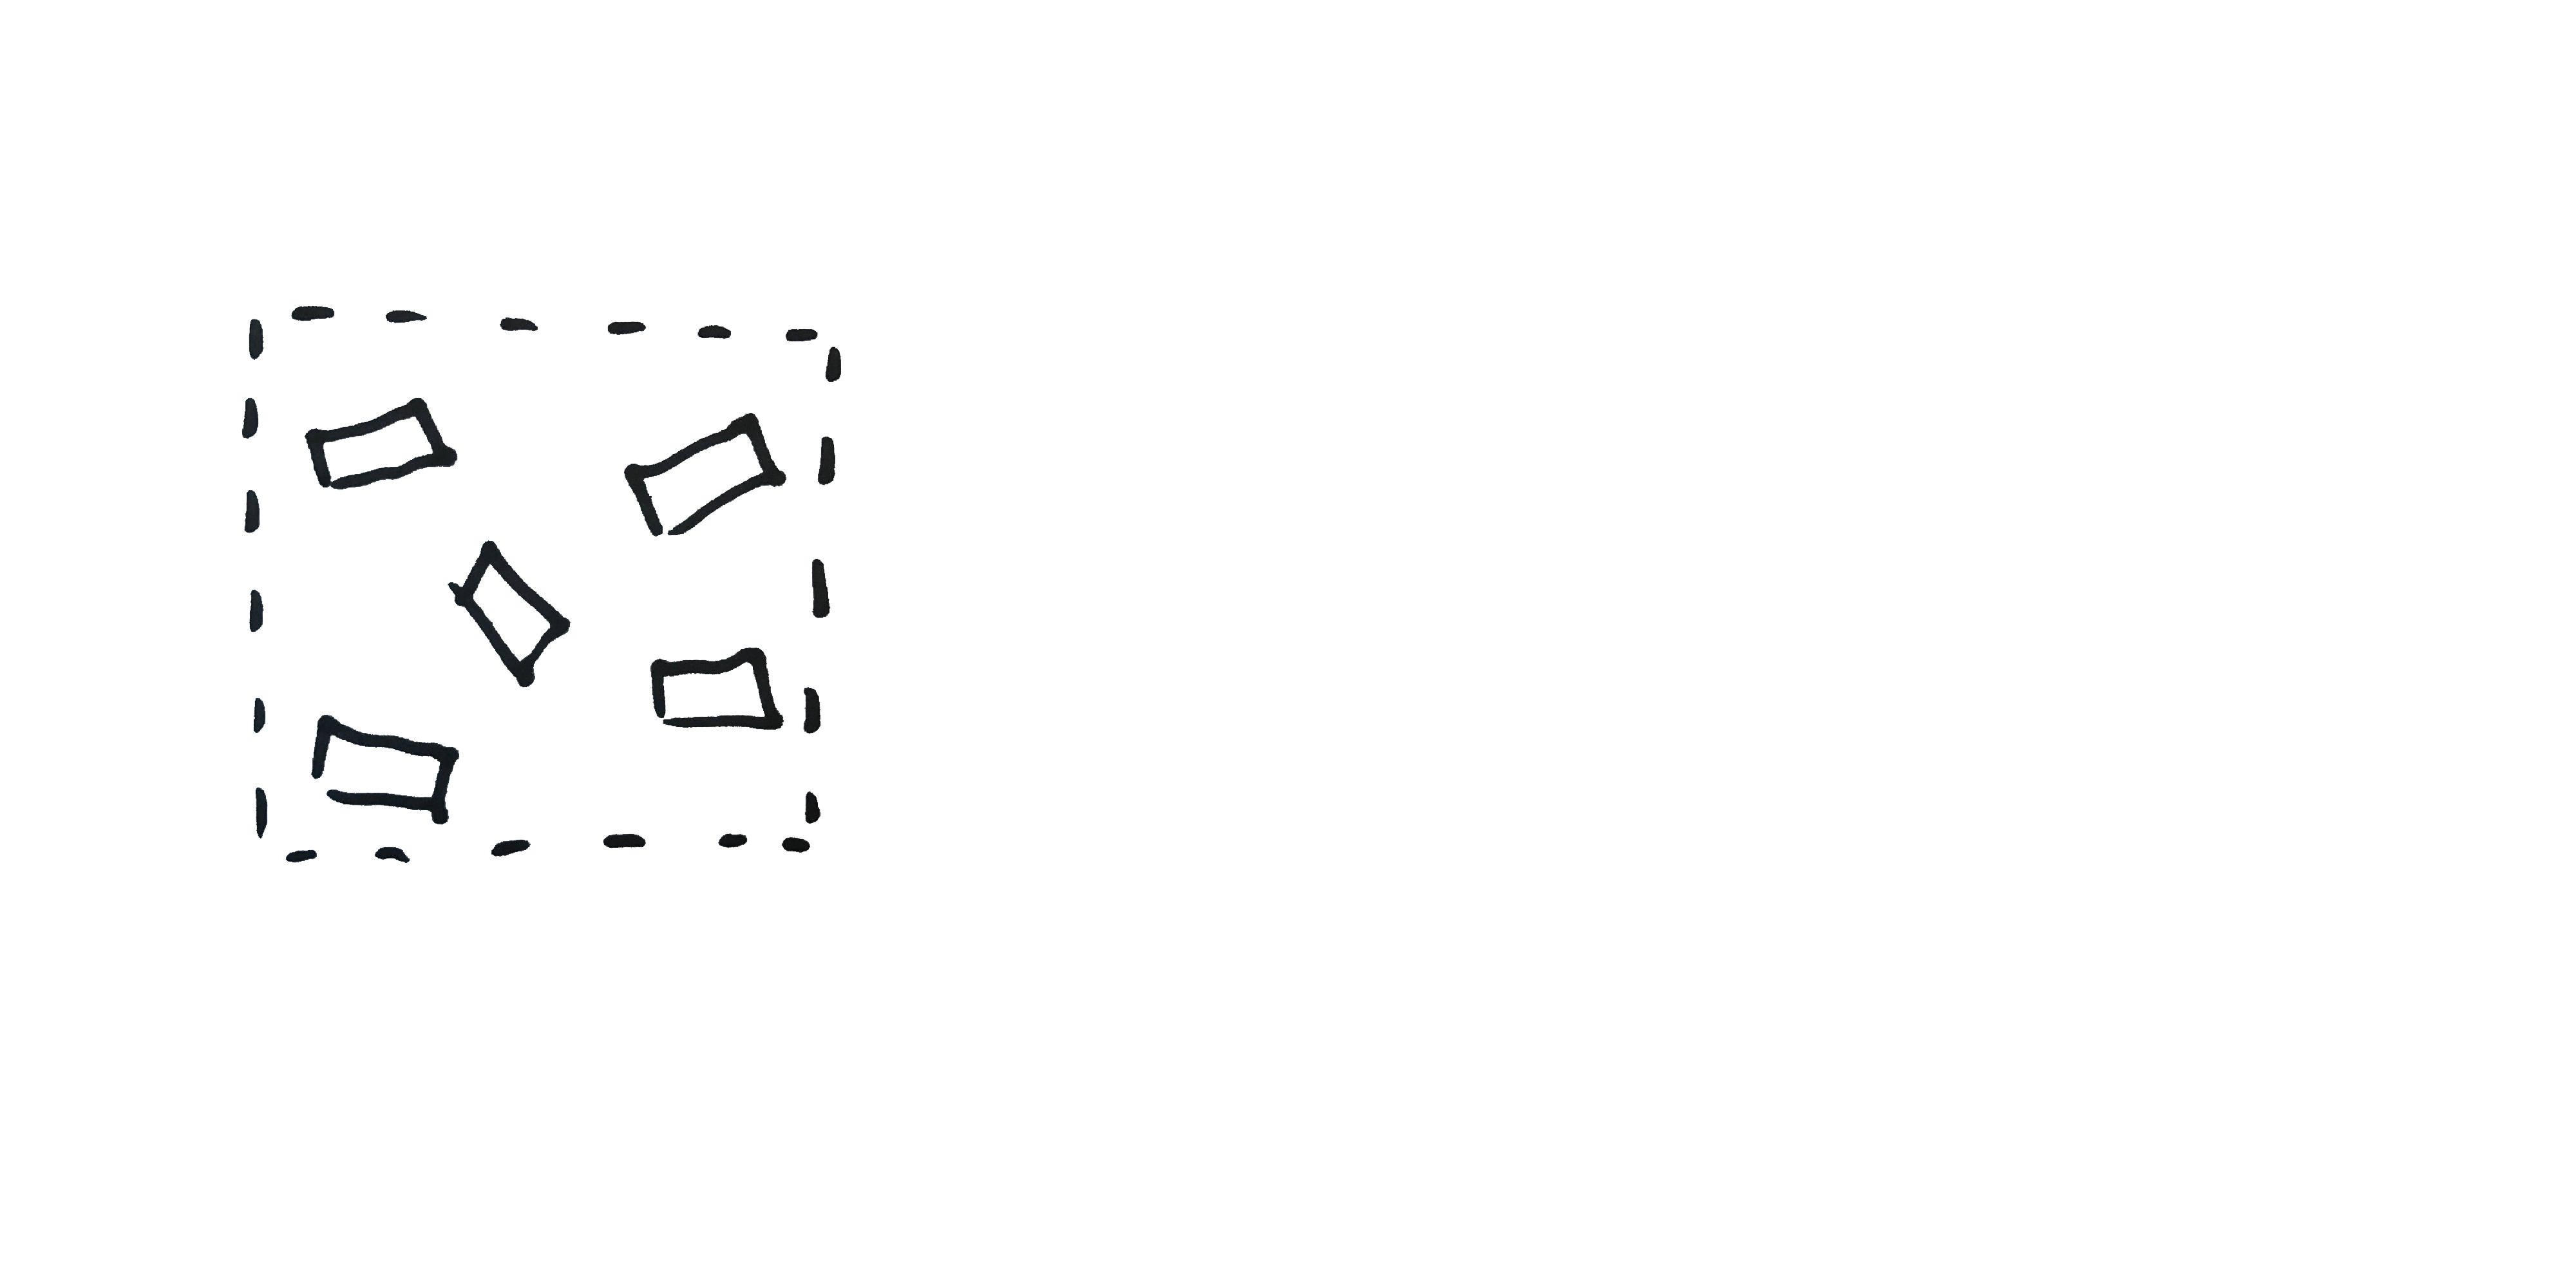
\includegraphics[width=6cm]{../assets/images/block_1.png} \\
\uncover<2->{
Those blocks are sequentially linked $\rightarrow $ blockchain \\
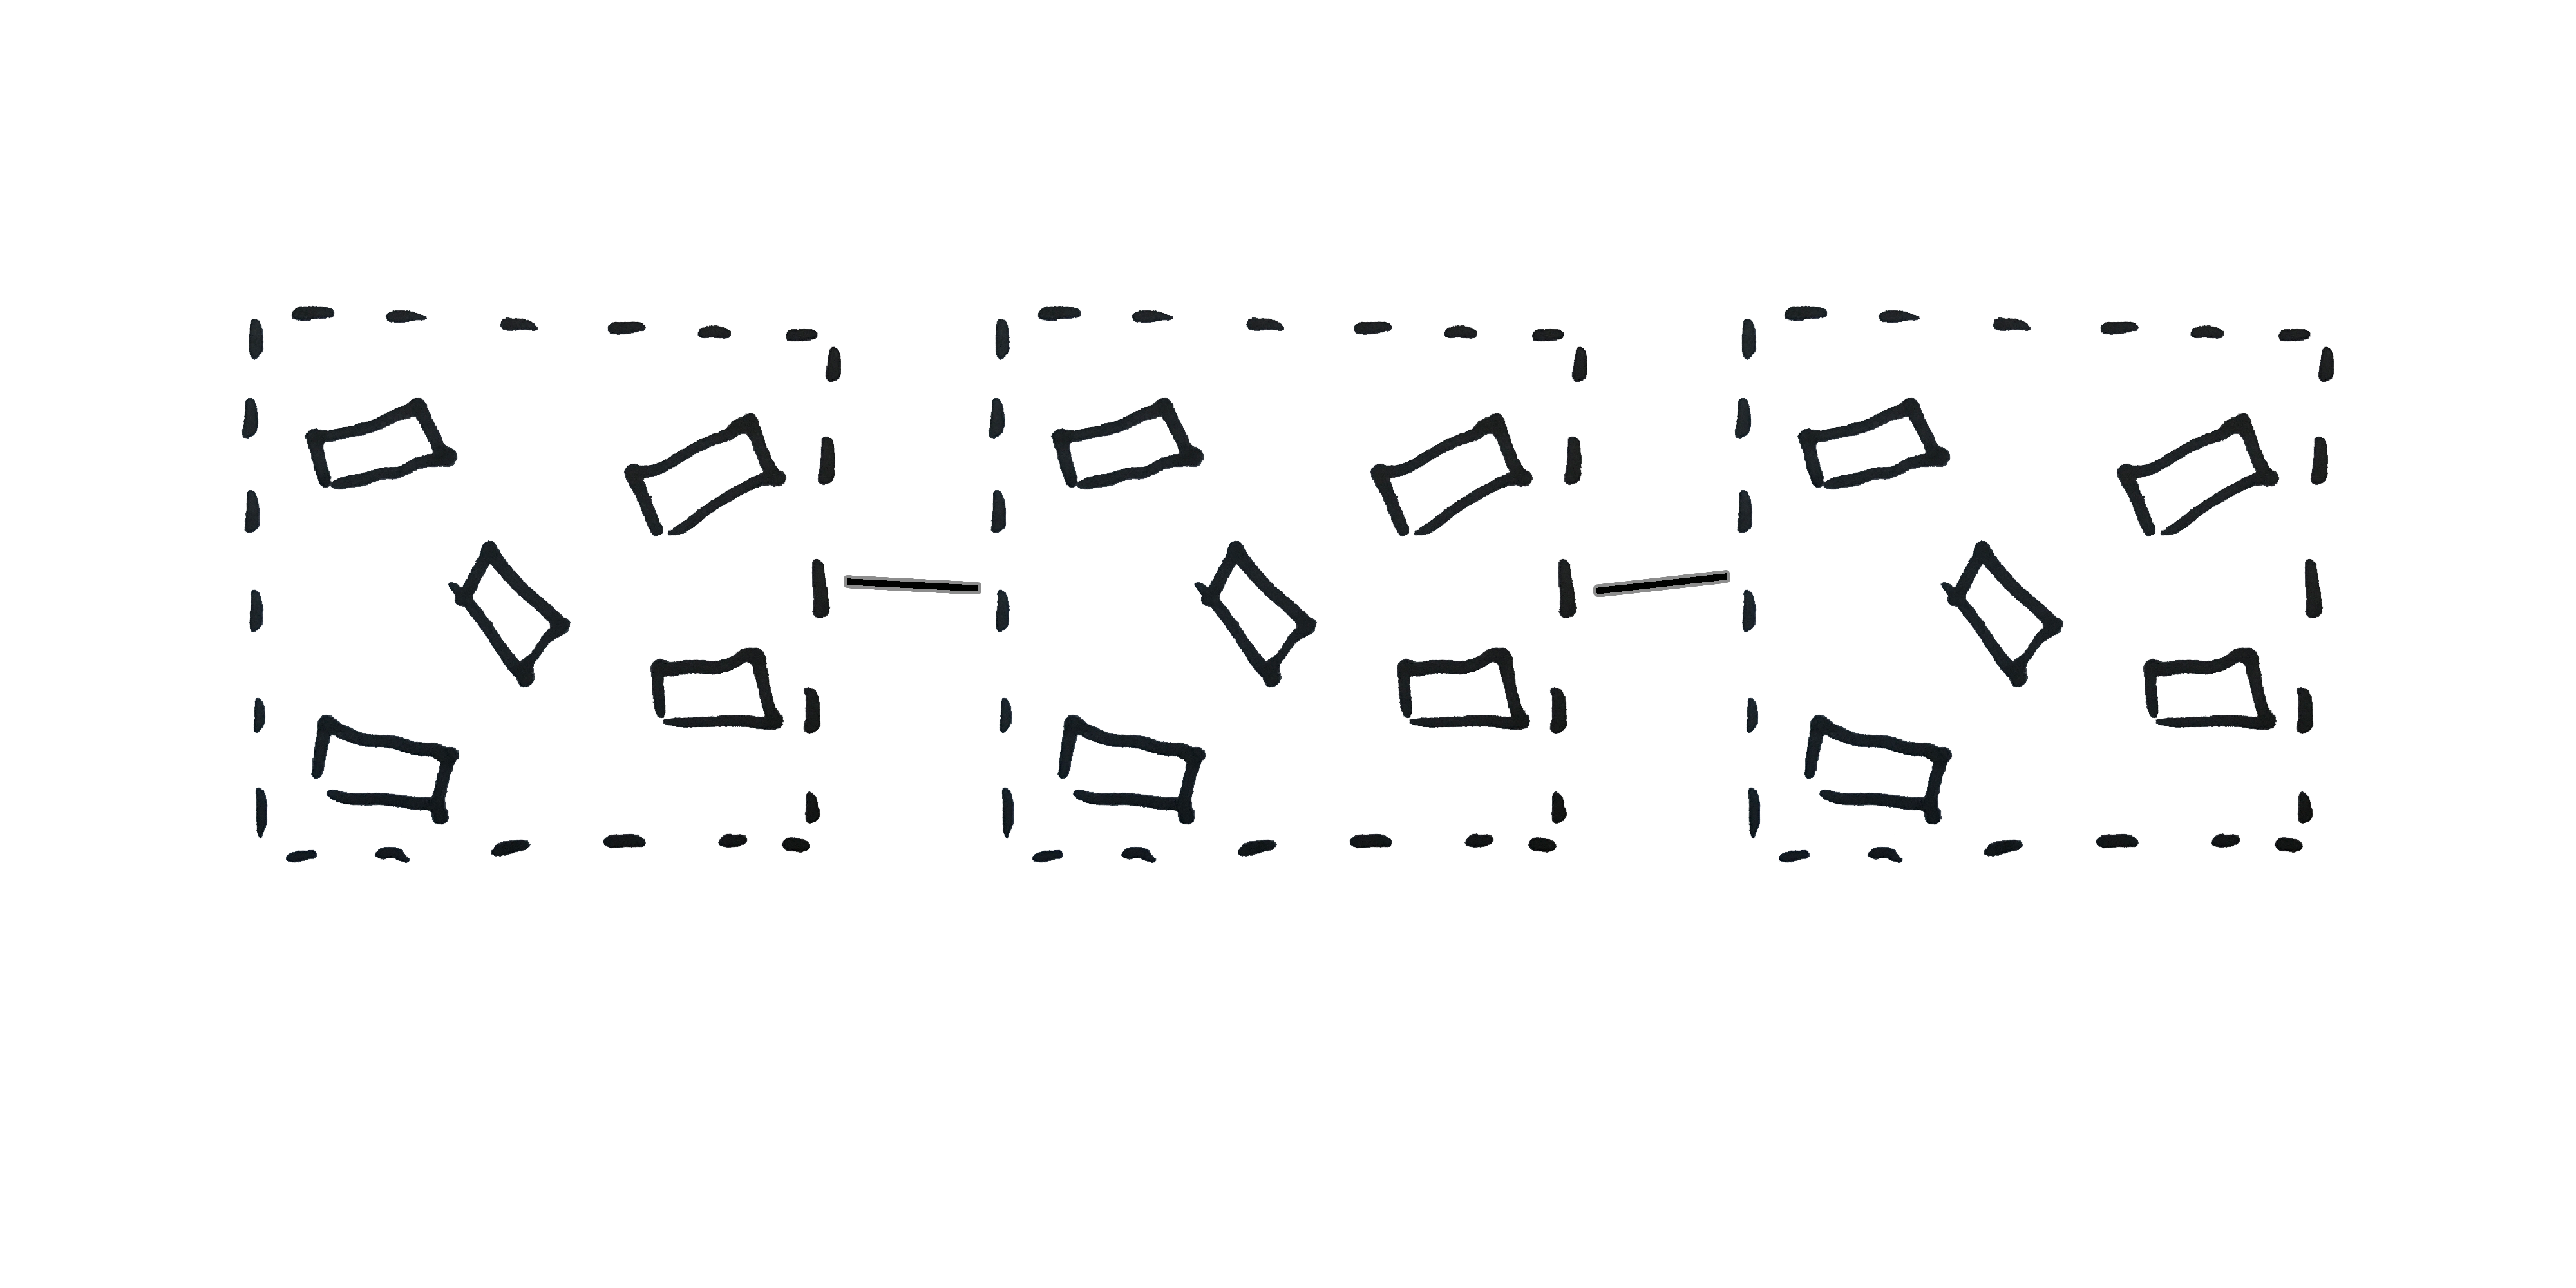
\includegraphics[width=6cm]{../assets/images/blocks_3.png}
} 
\end{frame}
%%%


%%%
\begin{frame}{Transaction consensus}
Who can broadcast a new block? \\ \vspace{1.5em}


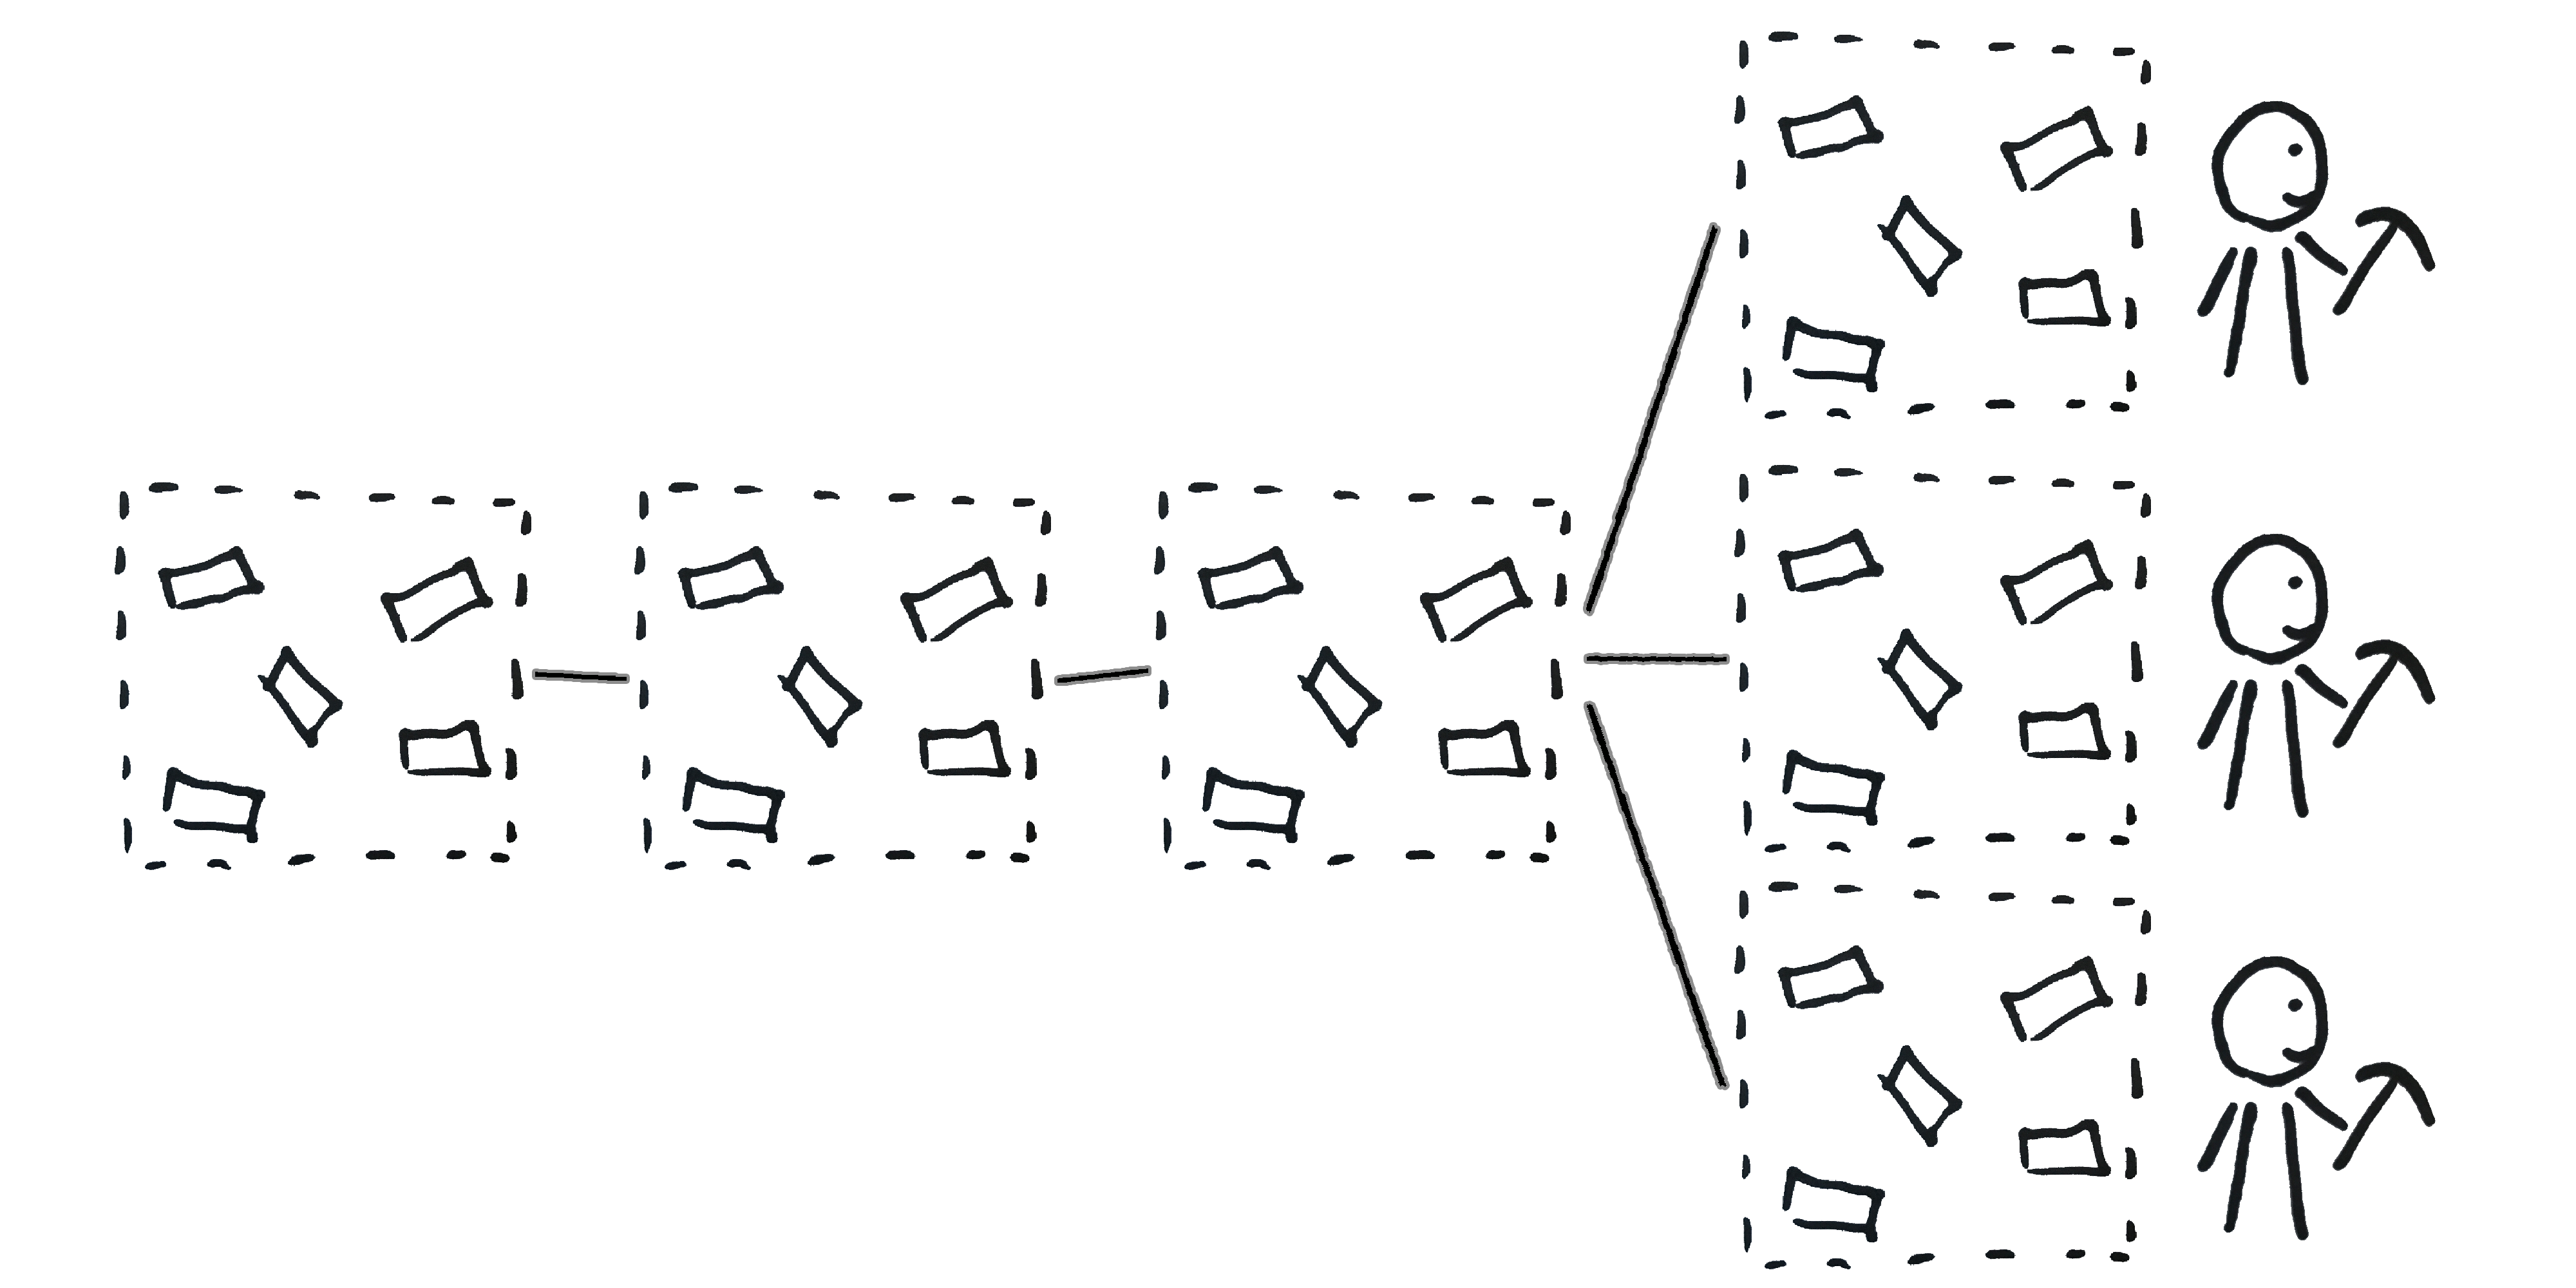
\includegraphics[width=9cm]{../assets/images/consensus_problem.png}

Possible consensus rules: \\
	\begin{itemize}
	\item central actor
	\item decentralized lottery (proof-of-work)
	\end{itemize} 
\end{frame}
%%%


%%%
\begin{frame}{Why do we need consensus?}

Double spend problem: \\

\begin{figure}[h!]
\center
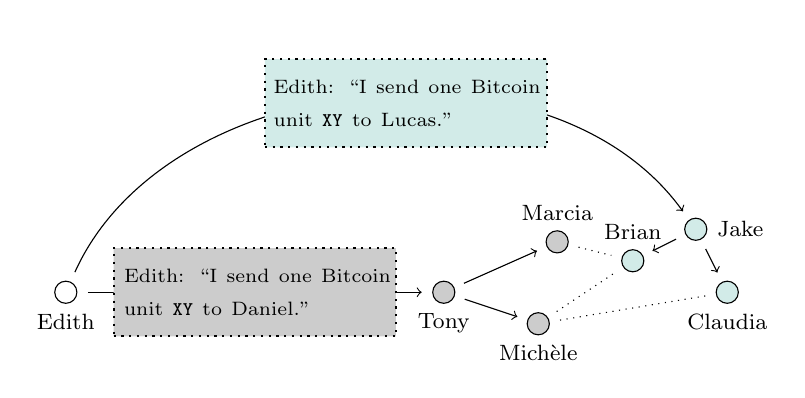
\begin{tikzpicture}[domain=-8:8, scale=0.8]
\coordinate (c1) at (0,0);
\coordinate (c2) at (6,0);
\coordinate (c3) at (7.8,0.8);
\coordinate (c4) at (7.5,-0.5);
\coordinate (c5) at (9,0.5);
\coordinate (c6) at (10,1);
\coordinate (c7) at (10.5,0);
\filldraw[draw=black,fill=white] (c1) circle (5pt) node[below=0.15cm,color=black]{\footnotesize{Edith}};
\filldraw[color=black,fill=black!20] (c2) circle (5pt) node[below=0.15cm,color=black]{\footnotesize{Tony}};
\filldraw[color=black,fill=black!20] (c3) circle (5pt) node[above=0.15cm,color=black]{\footnotesize{Marcia}};
\filldraw[color=black,fill=black!20] (c4) circle (5pt) node[below=0.15cm,color=black]{\footnotesize{Michèle}};
\filldraw[color=black,fill=highlight!50] (c5) circle (5pt) node[above=0.15cm,color=black]{\footnotesize{Brian}};
\filldraw[color=black,fill=highlight!50] (c6) circle (5pt) node[right=0.15cm,color=black]{\footnotesize{Jake}};
\filldraw[color=black,fill=highlight!50] (c7) circle (5pt) node[below=0.15cm,color=black]{\footnotesize{Claudia}};

\draw[shorten >=0.28cm,shorten <=0.28cm,->,color=black] (c1) to[bend left = 60] (c6);

\draw[shorten >=0.28cm,shorten <=0.28cm,->] (c1) to[] (c2);
\draw[shorten >=0.28cm,shorten <=0.28cm,->] (c2) to[] (c3);
\draw[shorten >=0.28cm,shorten <=0.28cm,->] (c2) to[] (c4);
\draw[shorten >=0.28cm,shorten <=0.28cm, dotted] (c3) to[] (c5);
\draw[shorten >=0.28cm,shorten <=0.28cm,dotted] (c4) to[] (c5);
\draw[shorten >=0.28cm,shorten <=0.28cm,dotted] (c4) to[] (c7);
\draw[shorten >=0.28cm,shorten <=0.28cm,->,color=black] (c6) to[] (c5);
\draw[shorten >=0.28cm,shorten <=0.28cm,->,color=black] (c6) to[] (c7);

\filldraw[fill=black!20,dotted,thick] (0.76,-0.7) -- (5.24,-0.7) -- (5.24,0.7) -- (0.76,0.7) -- (0.76,-0.7) node[midway, right=-0.0cm,text width=3.5cm]{\scriptsize{Edith: ``I send one Bitcoin unit \texttt{XY} to Daniel.''}};

\filldraw[fill=highlight!50,dotted,thick] (3.16,2.3) -- (7.64,2.3) -- (7.64,3.7) -- (3.16,3.7) -- (3.16,2.3) node[midway, right=-0.02cm,text width=3.5cm]{\scriptsize{Edith: ``I send one Bitcoin unit \texttt{XY} to Lucas.''}};

\end{tikzpicture}
\end{figure}

\end{frame}
%%%


%%%
\begin{frame}{Recap/Schlussfolie}

\end{frame}
%%%

\end{document}
